\documentclass{article}

\usepackage[final]{nips_2017}

\usepackage[utf8]{inputenc} % allow utf-8 input
\usepackage[T1]{fontenc}    % use 8-bit T1 fonts
\usepackage{hyperref}       % hyperlinks
\usepackage{url}            % simple URL typesetting
\usepackage{booktabs}       % professional-quality tables
\usepackage{amsfonts}       % blackboard math symbols
\usepackage{nicefrac}       % compact symbols for 1/2, etc.
\usepackage{microtype}      % microtypography
\usepackage{graphicx}
\usepackage{amsmath}
\usepackage{amssymb}
\usepackage{listings}
\usepackage{courier}
\usepackage{multirow}

\lstset{basicstyle=\ttfamily\footnotesize,breaklines=true}
\title{CSE 253 Programming Assignment 3 -- Convolution Neural Networks}

\author{
  Fanjin Zeng \\
  Computer Science and Engineering\\
  University of Califorina, San Diego\\
  \texttt{f1zeng@ucsd.edu} \\
   \And
   Xinyue Ou \\
   Computer Science and Engineering\\
   University of Califorina, San Diego \\
   \texttt{x1ou@ucsd.edu} \\
   \And
   He Qin \\
   Computer Science and Engineering\\
   University of Califorina, San Diego \\
   \texttt{h9qin@ucsd.edu} \\
   \And
   Yuhan Chen \\
   Computer Science and Engineering\\
   University of Califorina, San Diego \\
   \texttt{yuc143@ucsd.edu} \\
}

\begin{document}

\maketitle
\begin{abstract}
In this assignment, we first implemented convolutional neural networks for image classification, then explored transfer learning using the PyTorch framework. In our first experiment, our best network model reached 82.8\% prediction accuracy over test set. 

\end{abstract}

\section{Deep Convolution Network for Image Classification}
\subsection{Model Architecture}
Here, we present the 3 best networks as explained below. Specifically, we increase the depth of each network, and also try different layers like Conv, BatchNorm, ReLU, MaxPool, Dropout and FC etc.

Model 1 was inspired by the paper [2]. We set the depth to 13 conv layer, 1 fully connected, and one softmax layer. For the convolutional layers, the layer in the front uses 3x3 kernel to make full use of the locality information, while in the rear only 1x1 kernel is used to reduce the number of parameters.

For Model 2, we employ only 5 convolutional layer to build the network. It uses different size of the kernel for the convolution layer, ranging from 1x1 to 5x5. Dropout layer is also used in some convolution layer. 

Model 3 is the most simple network we build. It has only 4 convolutional layers, with BatchNorm, Maxpooling and ReLU.



\begin{table}[htbp]
\begin{minipage}[t]{0.48\textwidth}
  \centering
  \caption{Architecture of Model 1}
    \begin{tabular}{c|l}
    \multirow{3}[0]{*}{conv1} & Conv 3x3 @3x64 \\
          & BatchNorm2d \\
          & ReLU  \\
\hline \\ [-1.5ex]
    \multirow{3}[0]{*}{conv2} & Conv 3x3 @64x128 \\
          & BatchNorm2d \\
          & ReLU  \\
\hline \\ [-1.5ex]
    \multirow{3}[0]{*}{conv3} & Conv 3x3 @128x128 \\
          & BatchNorm2d \\
          & ReLU  \\
\hline \\ [-1.5ex]
    \multirow{4}[0]{*}{conv4} & Conv 3x3 @128x128 \\
          & BatchNorm2d \\
          & ReLU  \\
          & MaxPool 2x2 \\\hline \\ [-1.5ex]
    \multirow{3}[0]{*}{conv5} & Conv 3x3 @128x128 \\
          & BatchNorm2d \\
          & ReLU  \\\hline \\ [-1.5ex]
    \multirow{3}[0]{*}{conv6} & Conv 3x3 @128x128 \\
          & BatchNorm2d \\
          & ReLU  \\\hline \\ [-1.5ex]
    \multirow{4}[0]{*}{conv7} & Conv 3x3 @128x128 \\
          & BatchNorm2d \\
          & ReLU  \\
          & MaxPool 2x2 \\\hline \\ [-1.5ex]
    \multirow{3}[0]{*}{conv8} & Conv 3x3 @128x128 \\
          & BatchNorm2d \\
          & ReLU  \\\hline \\ [-1.5ex]
    \multirow{4}[0]{*}{conv9} & Conv 3x3 @128x128 \\
          & BatchNorm2d \\
          & ReLU  \\
          & MaxPool 2x2 \\\hline \\ [-1.5ex]
    \multirow{3}[0]{*}{conv10} & Conv 3x3 @128x128 \\
          & BatchNorm2d \\
          & ReLU  \\\hline \\ [-1.5ex]
    \multirow{3}[0]{*}{conv11} & Conv 1x1 @128x128 \\
          & BatchNorm2d \\
          & ReLU  \\\hline \\ [-1.5ex]
    \multirow{4}[0]{*}{conv12} & Conv 1x1 @128x128 \\
          & BatchNorm2d \\
          & ReLU  \\
          & MaxPool 2x2 \\\hline \\ [-1.5ex]
    \multirow{4}[0]{*}{conv13} & Conv 3x3 @128x128 \\
          & BatchNorm2d \\
          & ReLU  \\
          & MaxPool 2x2 \\\hline \\ [-1.5ex]
    fc    & Linear 512x10 \\\hline \\ [-1.5ex]
    sm    & Softmax \\
    \end{tabular}%
  \label{tab:1}%
\end{minipage}
\hfill
\begin{minipage}[t]{0.48\textwidth}
  \centering
  \caption{Architecture of Model 2}
    \begin{tabular}{c|l}
    \multirow{4}[0]{*}{conv1} & Conv 5x5 @3x128 \\
          & BatchNorm2d \\
          & ReLU  \\
          & MaxPool 2x2 stride2x2 \\
          \hline \\ [-1.5ex]
    \multirow{4}[0]{*}{conv2} & Conv 5x5 @128x256 \\
          & BatchNorm2d \\
          & ReLU  \\
          & MaxPool 2x2 stride2x2 \\\hline \\ [-1.5ex]
    \multirow{3}[0]{*}{conv3} & Conv 4x4 @256x512 \\
          & BatchNorm2d \\
          & ReLU  \\\hline \\ [-1.5ex]
    \multirow{4}[0]{*}{conv4} & Conv 2x2 @512x1024 \\
          & BatchNorm2d \\
          & ReLU  \\
          & Dropout p=0.5 \\\hline \\ [-1.5ex]
    \multirow{2}[0]{*}{conv5} & Conv 1x1 @1024x10 \\
          & BatchNorm2d \\\hline \\ [-1.5ex]
    fc    & Linear 90x10 \\\hline \\ [-1.5ex]
    sm    & Softmax \\
    \end{tabular}%
  \label{tab:2}%

 \vspace{10em}
       \centering
        \caption{Architecture of Model 3}
          \begin{tabular}{cl}
          \multirow{3}[0]{*}{conv1} & Conv 5x5 @3x16 \\
                & BatchNorm2d \\
                & ReLU  \\ \hline \\ [-1.5ex]
          \multirow{3}[0]{*}{conv2} & Conv 5x5 @16x64 \\
                & BatchNorm2d \\
                & ReLU  \\ \hline \\ [-1.5ex]
          \multirow{2}[0]{*}{fc1} & Linear 1600x120 \\
                & ReLU  \\ \hline \\ [-1.5ex]
          \multirow{2}[0]{*}{fc2} & Linear 120x84 \\
                & ReLU  \\\hline \\ [-1.5ex]
          fc3   & Linear 120x10 \\\hline \\ [-1.5ex]
          sm    & Softmax \\
          \end{tabular}%
        \label{tab:3}%
      
  \end{minipage}
  
\end{table}%

\newpage

\subsection{Optimization Technique}
\subsubsection{Batch Normalization}
When we fit a normalized input to the network, the gradient descent algorithm will undo the normalization in order to reduce the loss. This however will result in the shift of the underlying distribution of the data. As the input increase, some activation will reach the saturation regime except for those with small absolute value. Therefore, in order to get rid of the vanish of gradients, we use normalization to eliminate the dependency of the scale of parameters. It can then accelerate the process of training. [3]
\subsubsection{Xavier Intialization}
Xavier weight initialization is to let the variance of the input and the variance of the output from the forward phase remains the same.  To achieve this, Xavier initialization initializes the weights as a normal distribution with 0 mean and a variance to be \begin{align*}
Var(W) = \frac{1}{n_{in}}
\end{align*}

This proper initialization can help accelerate the training process

\subsubsection{Adam Optimizer}
We use adam optimizer for updating parameters, this usually helps to get faster convergence. It benefits from both AdaGrad and RMSProp
\subsection{Results and Analysis}

For the training, each model is trained for 30 epochs. We use early stop criterion based on the validation loss, if the validation loss keeps going up for 3 epochs, which means the model is overfitting, we stops the training at once. 

All the three models go through the 30 epochs without early stop. As the results show, the first model has the highest testing accuracy despite the training accuracy not as high as model 2, which shows that model 1 has a better generality compared to model 2. This may due the fact that deeper networks can learn more sophisticated inner representation. From the rising tendency of the testing and validation loss of Model 3, we can tell that this model is overfitting on the training data. This along with the low training accuracy show that shallow networks have defects in both generality and representing the data. 

\begin{table}[htbp]
  \centering
  \caption{Results}
    \begin{tabular}{l|lll}
          & Model 1 & Model 2 & Model 3 \\\hline \\ [-1.5ex]
    Train Accuracy & 92.1\%    & 96.1\% & 83.7\%     \\
    Validate Accuracy &   82.7\%  & 79.1\% & 63.4\%     \\
    Test Accuracy & 82.8\%    & 78.81\%  & 62.8\%    \\\hline \\ [-1.5ex]
    Train Loss & 0.0120    & 0.0117 & 0.0040     \\
    Validate Loss   & 0.0130    & 0.0133 & 0.0099   \\
    Test Loss & 0.0130    & 0.0131 & 0.0100     \\
    \end{tabular}%
  \label{tab:addlabel}%
\end{table}%



\begin{figure}[h]
\begin{minipage}{0.48\textwidth}
\centering
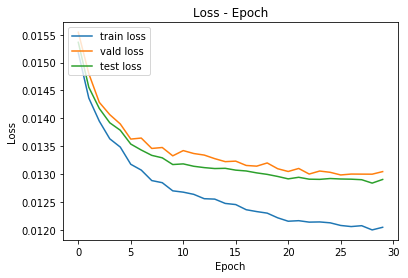
\includegraphics[width=\textwidth]{pics/1_loss.png}
\caption{Model 1 Loss}
\end{minipage}
\hfill
\begin{minipage}{0.48\textwidth}
\centering
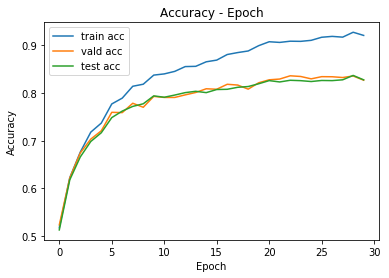
\includegraphics[width=\textwidth]{pics/1_acc.png}
\caption{Model 1 Accuracy}
\end{minipage}

\begin{minipage}{0.48\textwidth}
\centering
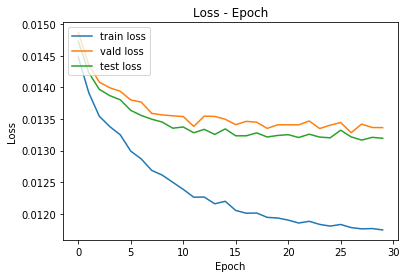
\includegraphics[width=\textwidth]{pics/2_loss.png}
\caption{Model 2 Loss}
\end{minipage}
\hfill
\begin{minipage}{0.48\textwidth}
\centering
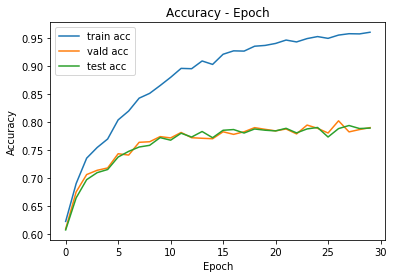
\includegraphics[width=\textwidth]{pics/2_acc.png}
\caption{Model 2 Accuracy}
\end{minipage}

\begin{minipage}{0.48\textwidth}
\centering
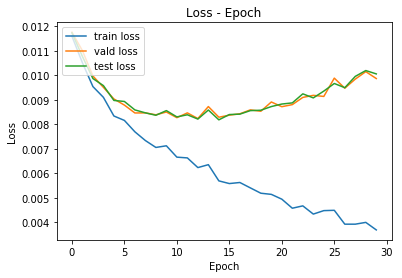
\includegraphics[width=\textwidth]{pics/t_loss.png}
\caption{Model 3 Loss}
\end{minipage}
\hfill
\begin{minipage}{0.48\textwidth}
\centering
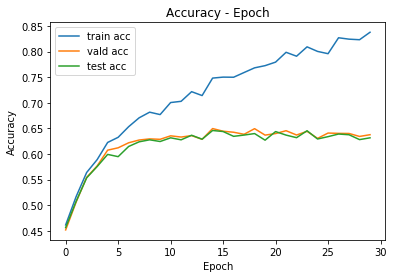
\includegraphics[width=\textwidth]{pics/t_acc.png}
\caption{Model 3 Accuracy}
\end{minipage}
\end{figure}
\subsection{Conclusion}
\begin{enumerate}
\item Deep network structure has better generality from train to test set, while shallw network structure tends to overfit, which usually has good accuracy on train set, but has poor accuracy on test set.
\item Depth of the network matters.
\item Techniques of batch-normalization, Xavier and Adam improves.

\end{enumerate}



\newpage
\section{Transfer Learning}

\newpage
\section{Summary}

\section{Contributions}



\section{References}
[1] Bishop, C. M., {\it Neural networks for pattern recognition}, Oxford: Oxford University Press, 2013. \\

[2] Hasanpour, Seyyed Hossein, et al. "Lets keep it simple, Using simple architectures to outperform deeper and more complex architectures." arXiv preprint arXiv:1608.06037 (2016). \\

[3]Ioffe, Sergey, and Christian Szegedy. "Batch normalization: Accelerating deep network training by reducing internal covariate shift." International conference on machine learning. 2015.\\

[4] PyTorch Tutorial, Training a classifier
 
 \url{http://pytorch.org/tutorials/beginner/blitz/cifar10_tutorial.html}

\end{document}